\subsection{Упражнение 1}

В разделе "Акустическая характеристика" умножение ДПФ сигнала на передаточную функцию соответствует круговой свертке, но в предположении периодичности сигнала. В результате, можно заметить, что на выходе, в начале фрагмента, слышна лишь нота, "затекшая" из конца этого фрагмента. Чтобы устранить эту проблему, нужно перед вычислением ДПФ добавить достаточно нулей в конце сигнала, эффекта "заворота" можно избежать. Урежем оба сигнала до 2^16 и добавим по нулю до 2^17.

\begin{lstlisting}[language=Python]
if not os.path.exists('180960__kleeb__gunshot.wav'):
    !wget https://github.com/AllenDowney/ThinkDSP/raw/master/code/180960__kleeb__gunshot.wav
    
from thinkdsp import read_wave

response = read_wave('180960__kleeb__gunshot.wav')

start = 0.12
response = response.segment(start=start)
response.shift(-start)

response.truncate(2**16)
response.zero_pad(2**17)

response.normalize()
response.plot()
decorate(xlabel='Time (s)')
\end{lstlisting}

\begin{figure}[H]
	\begin{center}
		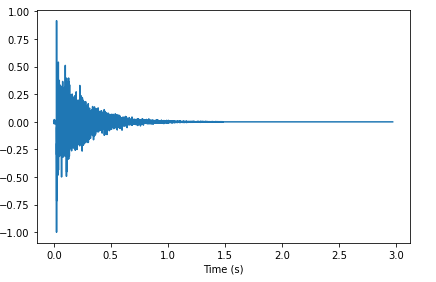
\includegraphics[scale=1]{fig/lab10/lab10_01.png}
		\caption{Сигнал}
	\end{center}
\end{figure}

Вычислим спектр:

\begin{lstlisting}[language=Python]
transfer = response.make_spectrum()
transfer.plot()
decorate(xlabel='Frequency (Hz)', ylabel='Amplitude')
\end{lstlisting}

\begin{figure}[H]
	\begin{center}
		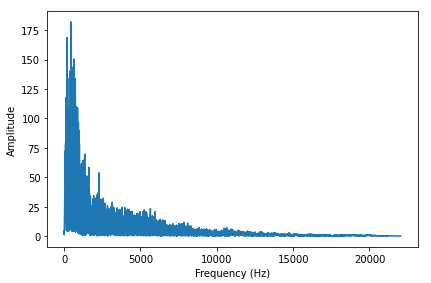
\includegraphics[scale=1]{fig/lab10/lab10_02.png}
		\caption{Спектр сигнала}
	\end{center}
\end{figure}

Теперь перейдём к самой записе:

\begin{lstlisting}[language=Python]
if not os.path.exists('92002__jcveliz__violin-origional.wav'):
    !wget https://github.com/AllenDowney/ThinkDSP/raw/master/code/92002__jcveliz__violin-origional.wav
    
violin = read_wave('92002__jcveliz__violin-origional.wav')

start = 0.11
violin = violin.segment(start=start)
violin.shift(-start)

violin.truncate(2**16)
violin.zero_pad(2**17)

violin.normalize()
violin.plot()
decorate(xlabel='Time (s)')
\end{lstlisting}

\begin{figure}[H]
	\begin{center}
		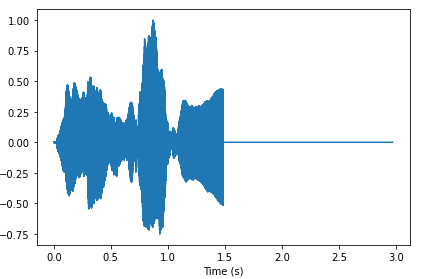
\includegraphics[scale=1]{fig/lab10/lab10_03.png}
		\caption{График сигнала}
	\end{center}
\end{figure}

Вычислим спектр:

\begin{lstlisting}[language=Python]
spectrum = violin.make_spectrum()
\end{lstlisting}

Теперь умножим ДПФ сигнала на передаточную функцию и преобразуем обратно в волну

\begin{lstlisting}[language=Python]
wave = (spectrum * transfer).make_wave()
wave.normalize()
wave.plot()
\end{lstlisting}

\begin{figure}[H]
	\begin{center}
		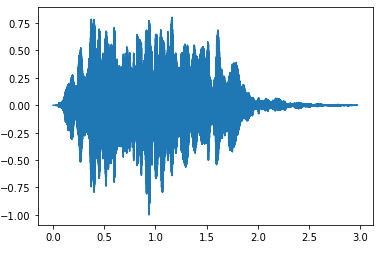
\includegraphics[scale=1]{fig/lab10/lab10_04.png}
		\caption{График сигнала}
	\end{center}
\end{figure}

Исходя из результатов видно, что проблему с лишней нотой удалось решить.

\subsection{Упражнение 2}

Смоделируйте двумя способами звучание записи в том пространстве, где была измерена импульсная харпактеристика, как свёрткой самой записи с импульсной характеристикой, так и умножением ДПФ записи на вычисленный фильтр, соотвествующий импульсной характеристики.

Воспользуемся характеристикой из учебного пособия, так как при взятии звуков с импульсной характеристикой с ресурса Open Air получается сильный шум.

\begin{lstlisting}[language=Python]
if not os.path.exists('stalbans_a_mono.wav'):
    !wget https://github.com/AllenDowney/ThinkDSP/raw/master/code/stalbans_a_mono.wav

response = read_wave('stalbans_a_mono.wav')

start = 0
duration = 5
response = response.segment(duration=duration)
response.shift(-start)

response.normalize()
response.plot()
decorate(xlabel='Time (s)')
\end{lstlisting}

\begin{figure}[H]
	\begin{center}
		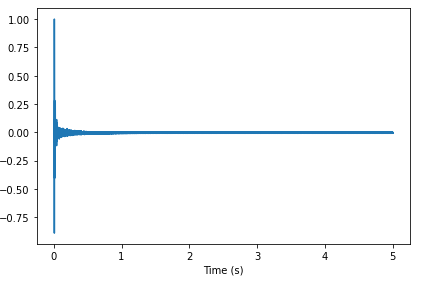
\includegraphics[scale=1]{fig/lab10/lab10_05.png}
		\caption{График загруженного сигнала}
	\end{center}
\end{figure}

ДПФ импульсной характеристики:

\begin{lstlisting}[language=Python]
transfer = response.make_spectrum()
transfer.plot()
decorate(xlabel='Frequency (Hz)', ylabel='Amplitude')
\end{lstlisting}

\begin{figure}[H]
	\begin{center}
		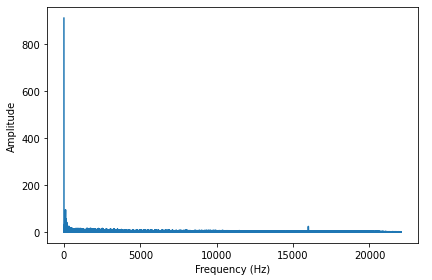
\includegraphics[scale=1]{fig/lab10/lab10_06.png}
		\caption{ДПФ импульсной характеристики}
	\end{center}
\end{figure}

В лагорифмическом масштабе:

\begin{lstlisting}[language=Python]
transfer.plot()
decorate(xlabel='Frequency (Hz)', ylabel='Amplitude',
         xscale='log', yscale='log')
\end{lstlisting}

\begin{figure}[H]
	\begin{center}
		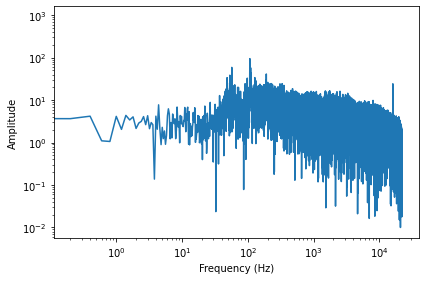
\includegraphics[scale=1]{fig/lab10/lab10_07.png}
		\caption{ДПФ импульсной характеристики в лагорифмическом масштабе} 
	\end{center}
\end{figure}

Теперь же смоделируем то, как будет звучать запись в пространстве

\begin{lstlisting}[language=Python]
if not os.path.exists('164718__bradovic__piano.wav'):
    !wget https://github.com/sergeyfedorov02/Telecom/raw/main/164718__bradovic__piano.wav
    
wave = read_wave('164718__bradovic__piano.wav')

start = 0.0
wave = wave.segment(start=start)
wave.shift(-start)

wave.truncate(len(response))
wave.normalize()
wave.plot()
decorate(xlabel='Time (s)')
\end{lstlisting}

\begin{figure}[H]
	\begin{center}
		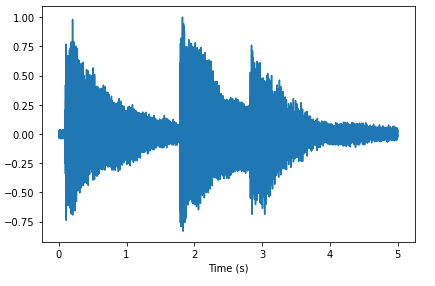
\includegraphics[scale=1]{fig/lab10/lab10_08.png}
		\caption{Сигнал звука пианино}
	\end{center}
\end{figure}

\begin{lstlisting}[language=Python]
wave.framerate

44100
\end{lstlisting}

Теперь вычислим ДПФ преобразование записи и урежем запись до той же длины, что и импульсная характеристика

\begin{lstlisting}[language=Python]
spectrum = wave.make_spectrum()

len(spectrum.hs), len(transfer.hs)
(110251, 110251)

spectrum.fs
array([0.00000e+00, 2.00000e-01, 4.00000e-01, ..., 2.20496e+04,
       2.20498e+04, 2.20500e+04])

transfer.fs
array([0.00000e+00, 2.00000e-01, 4.00000e-01, ..., 2.20496e+04,
       2.20498e+04, 2.20500e+04])
\end{lstlisting}

С использованием свертки:

\begin{lstlisting}[language=Python]
convolved2 = wave.convolve(response)
convolved2.normalize()
convolved2.make_audio()
\end{lstlisting}

Через умножение:

\begin{lstlisting}[language=Python]
out_wave = (spectrum * transfer).make_wave()
out_wave.normalize()
out_wave.plot()
\end{lstlisting}

\begin{figure}[H]
	\begin{center}
		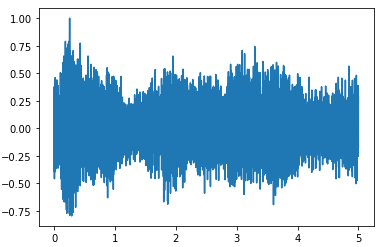
\includegraphics[scale=1]{fig/lab10/lab10_09.png}
		\caption{Полученный ДПФ} 
	\end{center}
\end{figure}


\subsection{Вывод}

В данной работе были рассмотренны основные позиции из теории сигналов и систем. Как примеры - музыкальная акустика. При описании линейных стационарных систем используется теорема о свёртке.